\section{Filter}
\subsection{Ablauf}
Ablauf von Filterung im Frequenzbereich. \textbf{Hinweis:} Das Multiplizieren mit $(-1)^{x+y} \xleftrightarrow{} F(u-M/2, v - N/2)$ ergibt ein zentieren des Bildes.
\begin{enumerate}[label=\alph*., nosep]
	\item An $M\times N$ image. $f$.
	\item Padding image $f$ of size $P \times Q$ to $f_p$
	\item Resulting of multiply $f_p$ by $(-1)^{x+y}$
	\item Spektrum von $F_p$
	\item Zentrierter Gauss LowPass Filter, $H$ mit der Grösse $P \times Q$
	\item Filter anwenden mit $g_p = H \cdot F_p$
	\item Multiplizieren mit $(-1)^{x+y}$ and den Realteil von der IDFT
	\item Zuschneiden von $g_p$ mit der Grösse $M\times N$ zu $g$
\end{enumerate}
\begin{center}
	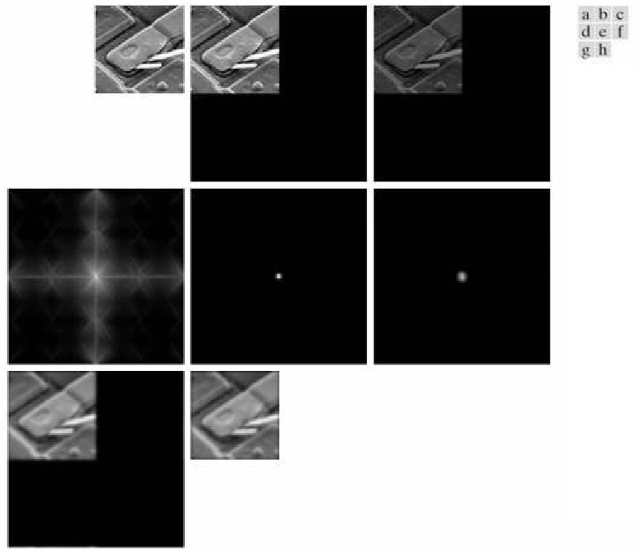
\includegraphics[width=\columnwidth]{Images/filtering}
\end{center}

\subsection{Smoothing}
Das bewirkt ein smoothing des Originalbildes. Blockierte alle Frequenzen ausserhalb des Kreises mit der Cutoff Freq. $D_0$.
\[
D(u,v) = \sqrt{(u-P/2)^2 + (v - Q/2)^2}
\]

\subsubsection{Ideal Lowpass}
Beim Ideal Lowpass Filter entstehen Ringe um die Objekte, da eine Kante zu einer Sinc Fuktion wird, welche Artefakte erzeugt. 
\begin{center}
	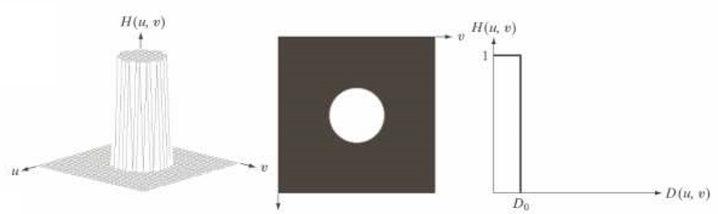
\includegraphics[width=\columnwidth]{Images/lp}
\end{center}

\[
H(u,v) = \begin{cases}
	1 & if D(u,v) \le D_0 \\
	0 & if D(u,v) \gt D_0 \\
\end{cases}
\]


\subsubsection{Butterworth Lowpass}
Je grössere die Ordnung $n$, desto grössere das Ringing.
\begin{center}
	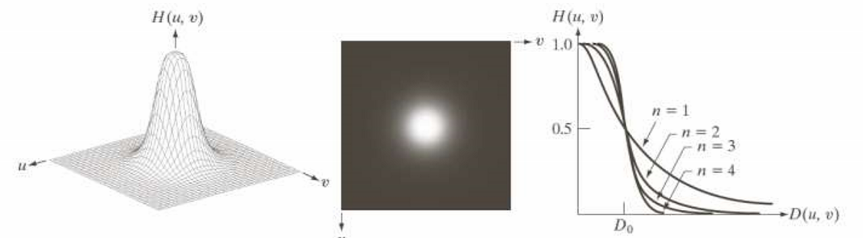
\includegraphics[width=\columnwidth]{Images/butterworth}
\end{center}
\[
H(u,v) = \frac{1}{1 + \left(D(u,v)/D_0\right)^{2n}}
\]

\subsubsection{Gaussion Lowpass}
Wenn $\sigma$ mit $D_0$ ersetzt wird, ist die Notation durchgängig. \textbf{Hinweis}: Bei der Cutoff Frequenz $D_0$ ist $H(u,v) = e^{-0.5} = 0.607$ und $H(0,0) = 1$.
\begin{center}
	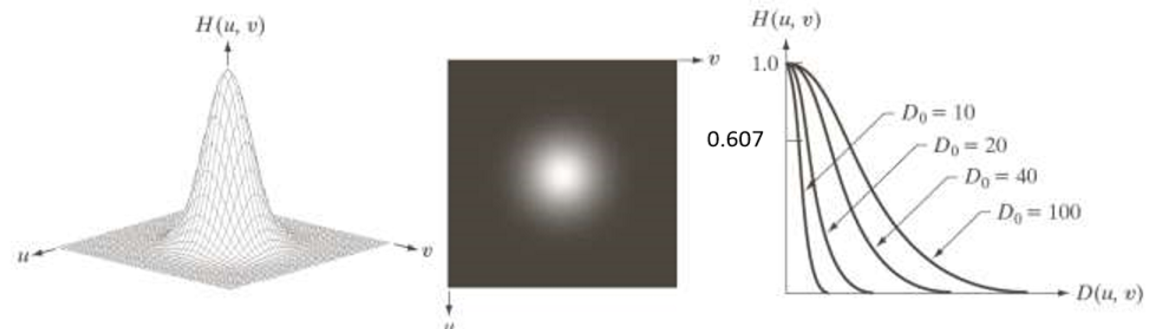
\includegraphics[width=\columnwidth]{Images/gaussian}
\end{center}

\[
H(u,v) = e^{-\frac{D^2(u,v)}{2\sigma^2}}
\]

\subsection{Sharpening}
Durch einen Hochpassfilter können Kanten geschärft werden:
\[
H(u,v) = 1- H_{LP}(u,v)
\]

\subsection{Homomorphic Filter}
Dabei wird der $\log$ vom Bild berechnet, um Multiplikationen mit Addition zu ersetzten. Das Bild wird mit dem Illumination-Reflection Model dargestellt $f(x,y) = \ln(i(x,y)) \cdot \ln (r(x,y))$. Mit DFT können diese nun einzeln in den Log Spatial Domain transformiert werden $Z(u,v) = F_i(u,v) + F_r(u,v)$. Das Anwenden der Filter geschiet einzeln und durch Rücktransofmieren und multiplizieren mit $e$ können effizientere Filter umgesetzt werden. Bei diesen Filtern wird gleichzeitig das Helligkeit normalisiert und den Kontrast erhöht.
\begin{center}
	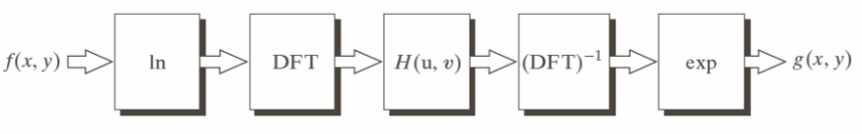
\includegraphics[width=\columnwidth]{Images/homorphobic}
\end{center}

